% !TEX encoding = UTF-8 Unicode
\section{Indoor-Lokalisierung}

In dieser Ausarbeitung wird die Indoor-Lokalisierung von Personen betrachtet. Lokalisierung von Objekten ist ebenfalls denkbar, jedoch werden in den heutzutage verwendeten Systeme hauptsächlich Personen lokalisiert. Im Folgenden werden die Begriffe der \textit{aktiven Lokalisierung} und \textit{passiven Lokalisierung} eingeführt und kurz erläutert.

\subsection{Aktive Lokalisierung}
Unter einer \textit{aktiven Lokaliserung} versteht man Lokalisierungsmethoden, welche eine aktive Mitwirkung der Teilnehmer benötigt. Zumeist bedeutet dabei eine aktive Mitwirkung das Tragen eines Gerätes, welches mit den Sensoren im Raum in einer bestimmten Art und Weise kommuniziert.\footnote{Vgl. Deak G.,  Curran K. \& Condell J., S. 1}\\
Solche Systeme sind weit verbreitet, jedoch können Teilnehmer in manchen Situationen keine Gerätschaften bei sich tragen. Ein Beispiel dafür wäre eine Brandsituation. Die Einsatzkräfte der Feuerwehr würden mit aktiven Lokalisierungsmethoden im Regelfall nicht die Opfer ausfindig machen können, was im schlimmsten Fall Menschenleben kosten könnte.\\
Darüber hinaus können Personen selbst kleinste sichtbare Sensoren als unkomfortabel empfinden, sodass in solchen Situationen zu \textit{passiven Lokalisierungsmethoden} gegriffen werden muss.\footnote{Vgl. Kivimäki T., Vuorela T., Peltola P. \& Vanhala J., S.1}
\subsection{Passive Lokalisierung}
Im Gegensatz zur \textit{aktiven Lokalisierungsmethoden} wird bei einer \textit{passiven Lokalisierung} (auch \textit{sensorlose Lokalisierung}) keine aktive Mitwirkung der Teilnehmer verlangt.\footnote{Vgl. ebd.} Ein großer Vorteil solcher Systeme ist die Benutzerfreundlichkeit, da keinerlei Gerätschaften sich am Teilnehmer selbst befinden müssen. Ebenfalls bieten \textit{sensorlose Lokaliserungsmethoden} neue Anwendungsbereiche wie zum Beispiel Alarmanlagen in Gebäuden. So können Einbrecher lokalisiert werden, was bei \textit{aktiver Lokalisierung} nur schwer vorstellbar ist.\\
Die folgende Abbildung zeigt nochmals die Unterkategorien von \textit{Indoor-Lokalisierung} auf:

\begin{figure}[H]
	\centering
	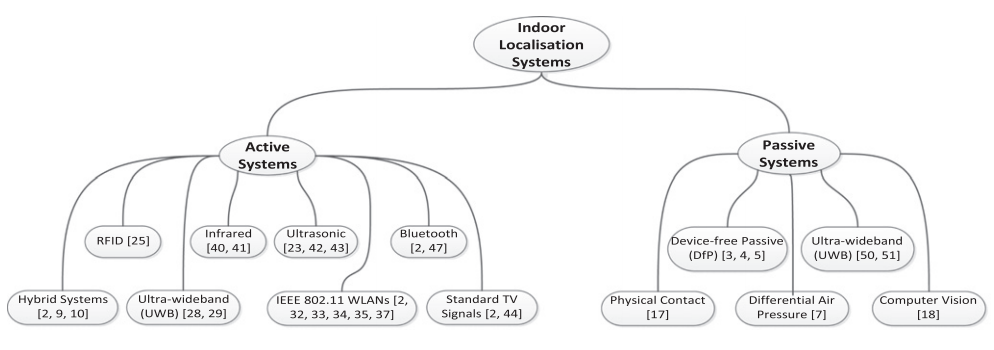
\includegraphics[scale=0.9]{pictures/indoor_loc}
	\caption{Unterkategorien von Indoor-Lokalisierung (Deak G.,  Curran K. \& Condell J., S. 2)}
\end{figure}

Im weiteren Verlauf wird jedes \textit{passive System} näher untersucht. Es wird die Funktionsweise sowie die Vor- und Nachteile des jeweiligen Systems erläutert.


\section{Sensorlose Indoor-Lokalisierung}
Schwanzgeil
\subsection{Radio Frequency Identification}
\subsubsection{Bla}
\subsubsection{BlaBla}
\subsection{Ultra Wideband}
\subsubsection{Bla}
\subsubsection{BlaBla}
\subsection{Infrarot-Sensoren (besser an die Abbildung halten) vielleicht also Air Pressure}
\subsubsection{Bla}
\subsubsection{BlaBla}
\subsection{Drucksensoren}
\subsubsection{Bla}
\subsubsection{BlaBla}
\subsection{Computer-Vision}
\subsubsection{Bla}
\subsubsection{BlaBla}

\subsection{Fazit}

\subsection{Ausblick}

\newpage

\section{Quellenverzeichnis}
\subsection*{Literaturquellen}
\begin{itemize}[leftmargin=*]
\item[] \textbf{Sample}
\end{itemize}
\subsection*{Sonstige Quellen}
\begin{itemize}[leftmargin=*]
\item[] \textbf{Ehrlich, I.}: Indoor Localization, Online unter URL: \url{http://ifgi.uni-muenster.de/~muellerj/lbs06/proceedings/3-IndoorLocalization.pdf}
\item[] \textbf{Deak G., Curran K. \& Condell J.} A survey of active and passive indoor localisation systems, Online unter URL : \url{http://scisweb.ulster.ac.uk/~kevin/comcomsurvey.pdf}
\item[] \textbf{Kivimäki T., Vuorela T., Peltola P. \& Vanhala J.}: Indoor Localization, Online unter URL: \url{http://www.sersc.org/journals/IJSH/vol8_no1_2014/9.pdf}
\end{itemize}
\end{figure}